\section{Ergebnisse}

\subsection{Beispielanwendung: Virtuelle Patientendatenbank}
\label{virtpat}

Um die Veränderungen von Kodes über die Versionen der ICD-10-GM beispielhaft darzustellen, wurde ein Prozess implementiert, der zufällige Patientendaten generiert. Hierzu werden Kodes der verschiedenen Versionen ausgewählt und zu mehreren virtuellen Patienten zusammengefügt. Abgespeichert werden jeweils: Kode und Titel, sowie die Angabe, ob der Kode zu anderen Versionen Umsteiger hat. Das passiert im JSON-Format, damit auf der Patienten-Seite auch nach Kode und Titel gesucht werden kann. Abhängig von der Information, ob Umsteiger vorhanden sind, erscheint neben dem Kode eine Lupe. 

Hier beispielhaft die mit 20.000 Patienten gefüllte Datenbank. Gesucht wird nach allen Kodes, die den Titel "`Lähmungssyndrome"' enthalten. H40.5 hat keine Umsteiger und daher keine Lupe.

\begin{figure}[H]
    \centering
    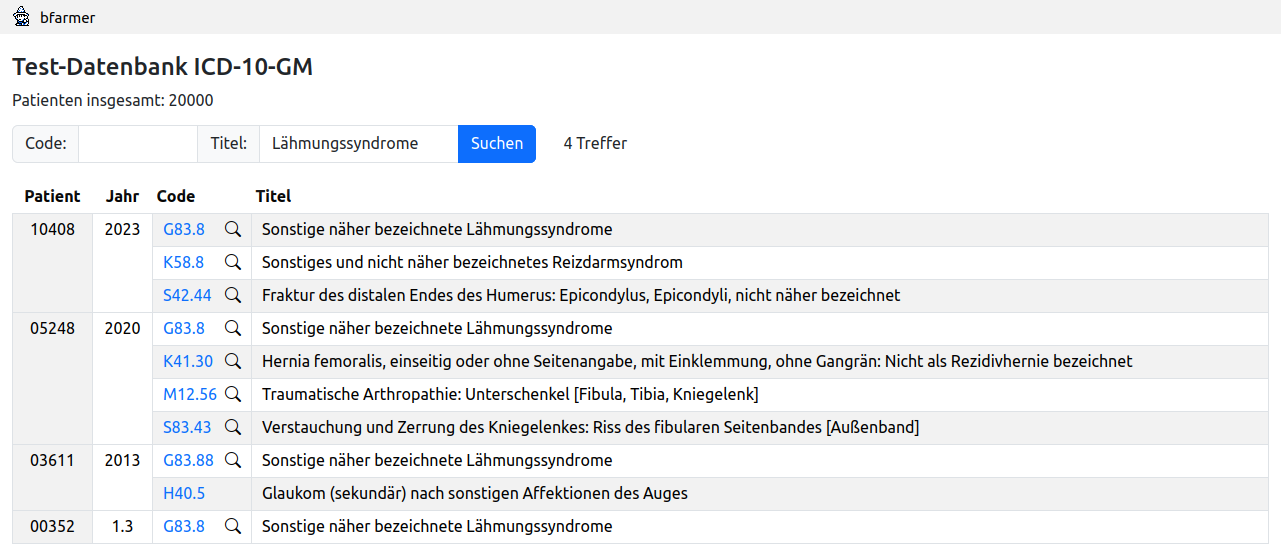
\includegraphics[width=\linewidth]{../img/patients_screenshot.png}
    \vspace{-1em}\caption{Virtuelle Patientendatenbank}
\end{figure}

Alle anderen Kodes haben Umsteiger und diese können per Klick auf die Lupe angezeigt werden. Hier zum Beispiel der G83.8 der Version 1.3. Das Modal wird per AJAX geladen. 

\begin{figure}[H]
    \centering
    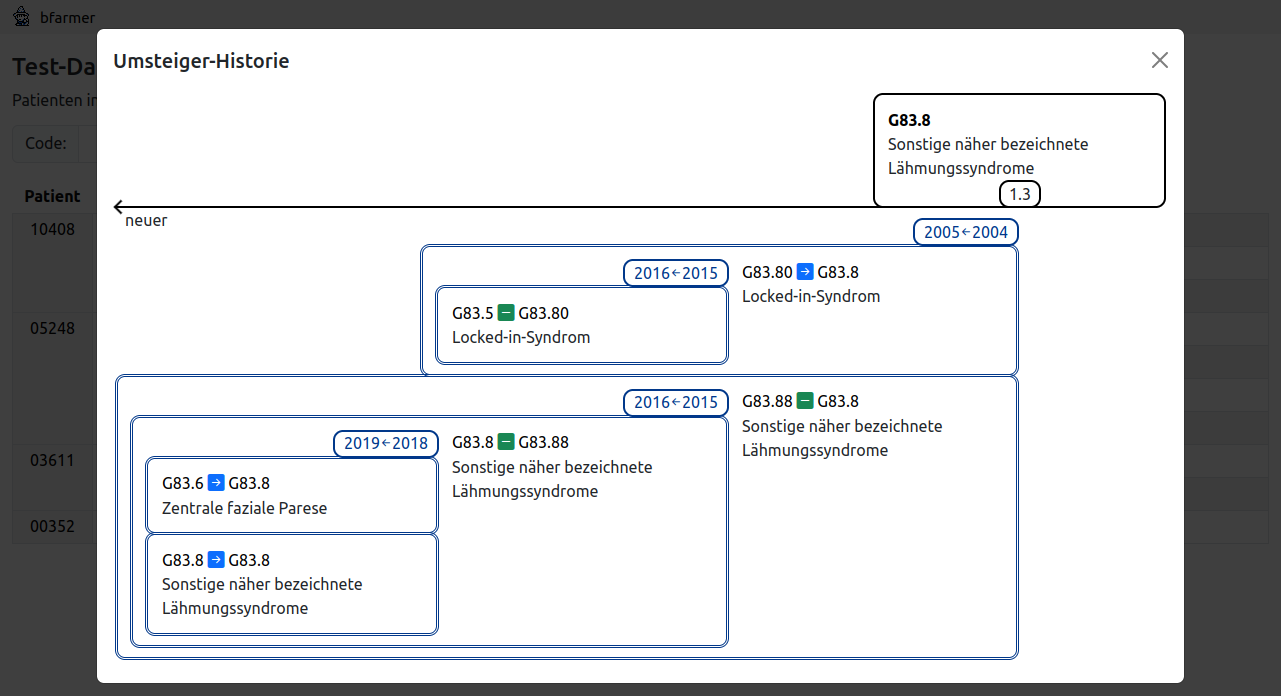
\includegraphics[width=\linewidth]{../img/umsteiger_screenshot.png}
    \vspace{-1em}\caption{Umsteiger von G83.8 Version 1.3}
    \label{hori-umst}
\end{figure}

Diese Funktionalität kann interoperabel verwendet werden. Vorausgesetzt ist, dass der Server "`Cross-Origin Resource Sharing"' auf der Umsteiger-API erlaubt. Dafür muss ein Response-Header gesetzt sein: \texttt{Access-Control-Allow-Origin:*}.

Wenn das der Fall ist, kann die Umsteiger-Suche mit folgenden Schritten auch auf einer anderen Seite angezeigt werden:

1. \bfarmer-Stylesheet im \texttt{<head>} laden:
\begin{Code}
<link rel="stylesheet" href="http://127.0.0.1:8000/build/app.css">
\end{Code}

2. Stylesheets für Bootstrap und Bootstrap-Icons im \texttt{<head>} laden:
\begin{Code}
<link
  rel="stylesheet" crossorigin="anonymous"
  href="https://cdn.jsdelivr.net/npm/bootstrap@5.3.3/dist/css/bootstrap.min.css"  
  integrity=
"sha384-QWTKZyjpPEjISv5WaRU9OFeRpok6YctnYmDr5pNlyT2bRjXh0JMhjY6hW+ALEwIH"
>
<link
  rel="stylesheet" href=
"https://cdn.jsdelivr.net/npm/bootstrap-icons@1.11.3/font/bootstrap-icons.min.css"
>
\end{Code}

\newpage

3. Bootstrap-JavaScript im \texttt{<head>} laden:
\begin{Code}
<script crossorigin="anonymous"
  src=
"https://cdn.jsdelivr.net/npm/bootstrap@5.3.3/dist/js/bootstrap.bundle.min.js"
  integrity=
"sha384-YvpcrYf0tY3lHB60NNkmXc5s9fDVZLESaAA55NDzOxhy9GkcIdslK1eN7N6jIeHz">
</script>
\end{Code}

4. jQuery-Library im \texttt{<head>} laden:
\begin{Code}
<script src="https://ajax.googleapis.com/ajax/libs/jquery/3.7.1/jquery.min.js">
</script>
\end{Code}

5. AJAX-Funktion im \texttt{<head>} bereitstellen:
\begin{Code}
<script>   
  window.ajaxUmsteigerSearchHistory = function(system, version, code) {
    $.get('http://127.0.0.1:8000/umsteiger-suche-api?s=' + system + '&v=' + version + '&c=' + code, function(data) {
      $('#edit-modal .modal-content').html(data);
      $('#edit-modal .modal-title').html('Umsteiger-Historie');
    });
  }
</script>
\end{Code}   

6. Leeres Modal im \texttt{<body>} platzieren:
\begin{Code}
<div class="modal fade" id="edit-modal" tabindex="-1" aria-hidden="true">
  <div class="modal-dialog"><div class="modal-content"></div></div>
</div>
\end{Code}   

7. AJAX-Funktion beim Kode verlinken:
\begin{Code}
<a class="umsteiger-search-link" href="" data-bs-toggle="modal" data-bs-target="#edit-modal"
  onclick="ajaxUmsteigerSearchHistory('icd10gm','1.3','G83.8')">
  Test G83.8 1.3
</a>
\end{Code}   

